\documentclass[9.5pt]{article}
\author{Lawrence Liu}
\usepackage{subcaption}
\usepackage{graphicx}
\usepackage{amsmath}
\usepackage{pdfpages}
\newcommand{\Laplace}{\mathscr{L}}
\setlength{\parskip}{\baselineskip}%
\setlength{\parindent}{0pt}%
\usepackage{xcolor}
\usepackage{listings}
\definecolor{backcolour}{rgb}{0.95,0.95,0.92}
\usepackage{amssymb}
\usepackage{empheq}

\newcommand*\widefbox[1]{\fbox{\hspace{2em}#1\hspace{2em}}}
\lstdefinestyle{mystyle}{
    backgroundcolor=\color{backcolour}}
\lstset{style=mystyle}

\usepackage{geometry}
\geometry{a4paper,margin=0.25in}
\begin{document}
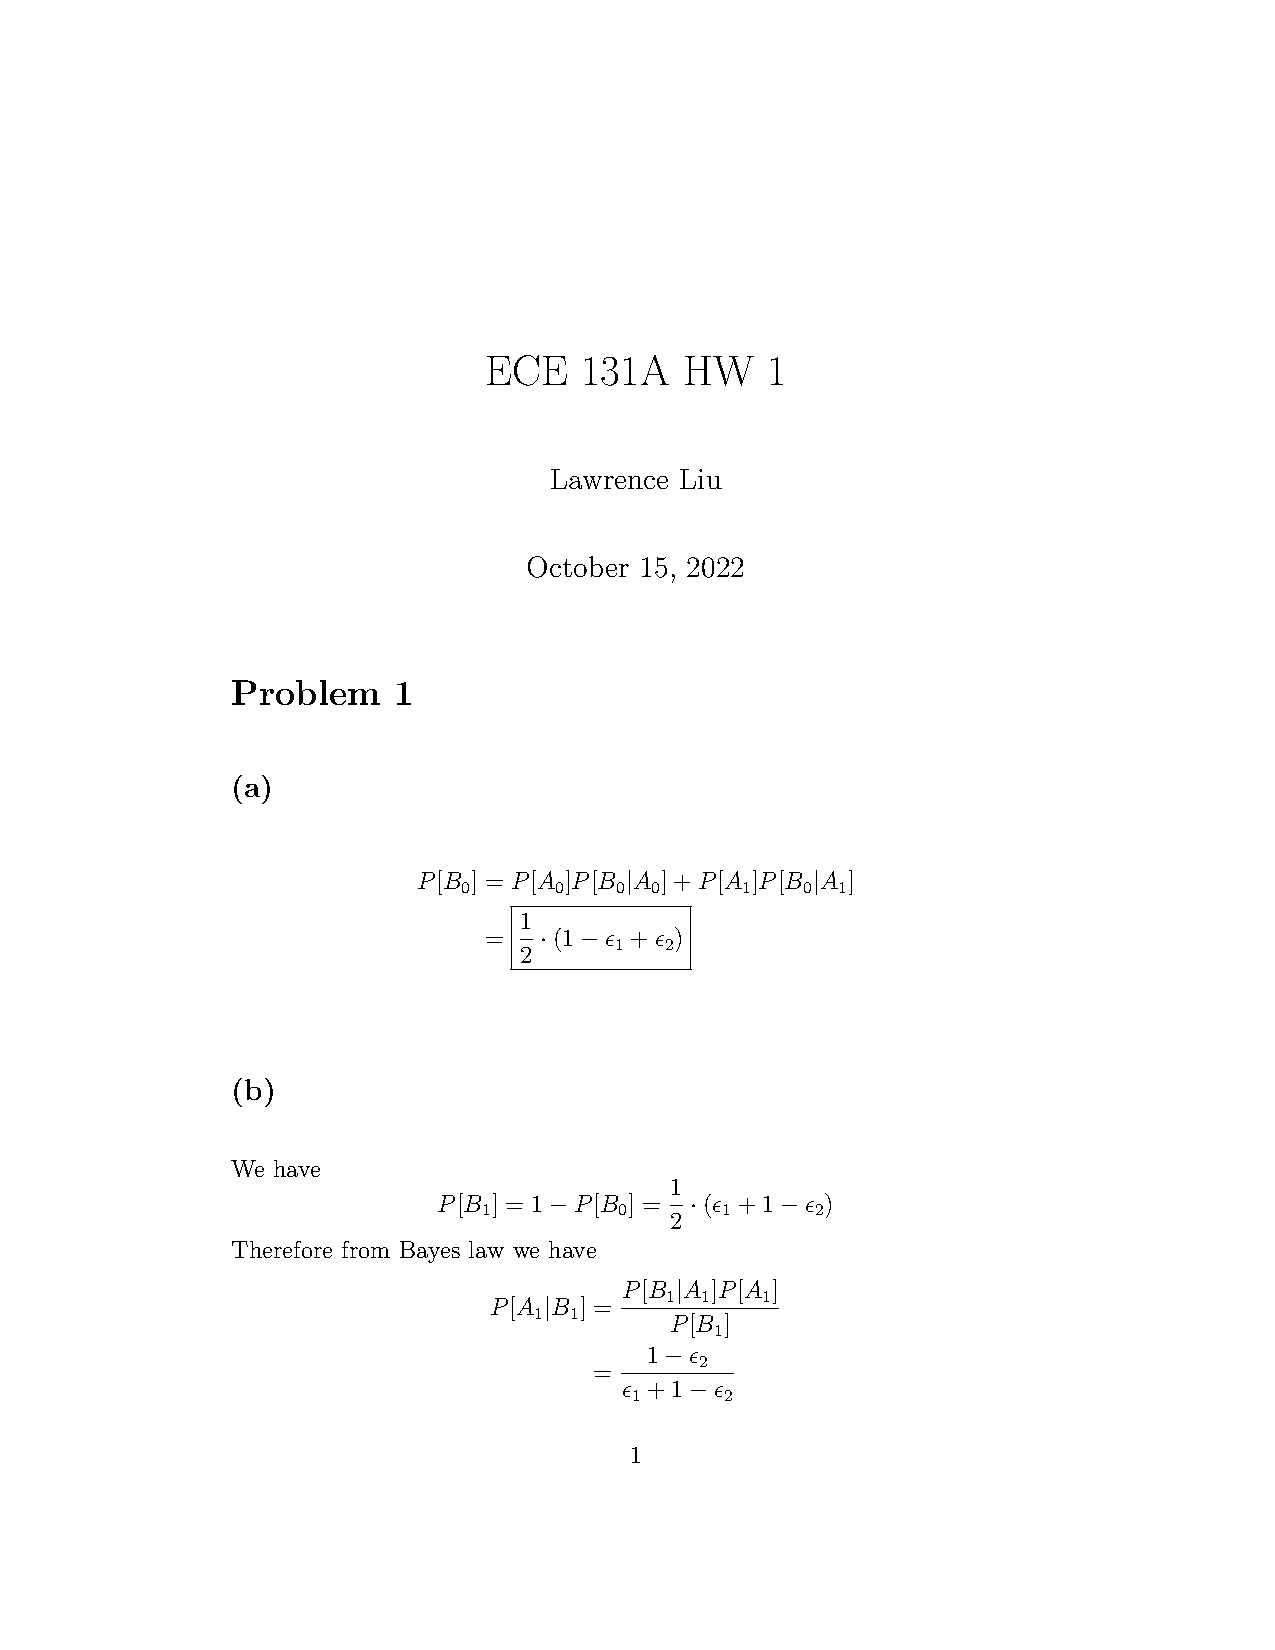
\includepdf[pages=-]{"../Midterm/file.pdf"}
\underline{\textbf{Countinous Random Variable}}\\
A continous random variable is a random variable that can take any value in a range of values. 
We can define a continous random variable by its probability density function $f_X(x)$, 
some important properites fo the pdf is $f_X(x) \geq 0$ and $\int_{\Omega'} f_X(x) dx = 1$. We also
have that $P([x,x+\delta])=f_X(x)\delta$ as $\delta \rightarrow 0$. and $P(X \in A) = \int_A f_X(x) dx$.\\
\underline{\textbf{Bayes Rule}}\\
For two discrete random variables $X$ and $Y$, the Bayes rule is given by $P(Y=y|X=x) = \frac{P(X=x|Y=y)P(Y=y)}{P(X=x)}$.
For two continous random variables $X$ and $Y$, the Bayes rule is given by $f(Y=y|X=x) = \frac{f(X=x|Y=y)f(Y=y)}{f(X=x)}$.
And if $X$ is a continous random variable and $Y$ is a discrete random variable, the Bayes rule is given by $P(Y=y|X=x) = \frac{f(X=x|Y=y)P(Y=y)}{f(X=x)}$
and $f(X=x|Y=y) = \frac{P(Y=y|X=x)f(X=x)}{P(Y=y)}$.\\
\underline{\textbf{Cumualtive Distribution Functions}}\\
For a discrete random variables the CDF is defined as $F_X(x) = P(X \leq x) = \sum_{x_i \leq x} p(x_i)$.
For a continous random variable the CDF is defined as $F_X(x) = P(X \leq x) = \int_{-\infty}^x f_X(x) dx$.
The CDF has the following properites, it is monotonically non decreasing, 
as $x\to -\infty$ $F_X(x) \to 0$ and as $x \to \infty$ $F_X(x) \to 1$.
We can obtain the PDF from the CDF by taking the derivative of the CDF, ie:
$f_X(x)=\frac{d}{dx}F_X(x)$. Likewise for a discrete random variable we can obtain the PMF
from the cdf with $p_X(x)=F_X(x)-F_X(x-1)$.\\
\underline{\textbf{Expectation and Covariance(cont')}}\\
For a continous random variable we can define the expectation as:
$\mathbb{E}[X] = \int_{-\infty}^{\infty} xf_X(x) dx$, and more generally
$\mathbb{E}[g(X)] = \int_{-\infty}^{\infty} g(x)f_X(x) dx$. We have the following 
properties of the expectation: $\mathbb{E}[\mathbb{E}[X|Y]]=\mathbb{E}[X]$. And 
a similar formula for variance $Var(X)=\mathbb{E}[Var(X|Y)]+var(E[X|Y])$.
An interesting result of this is that given $X_1,X_2,..$ that 
are iid, and another random variable that takes nonnegative integer values $N$ independent 
of $X_1,X_2,..$ we have that $Var(\sum_{i=1}^N X_i) = E[N]Var(X)+E^2[X]Var(N)$
and $E[\sum_{i=1}^N X_i] = E[N]E[X]$.
We can also define the covariance of two random variables $X$ and $Y$ as $Cov(X,Y)=\mathbb{E}[(X-\mathbb{E}[X])(Y-\mathbb{E}[Y])]=\mathbb{E}[XY]-\mathbb{E}[X]\mathbb{E}[Y]$.
We have that $Var(\sum_{i=1}^n iX_i)=\sum_{i=1}^n Var(X_i)+\sum_{i=1}^n\sum_{j=1, i\neq j}^n Cov(X_i,X_j)$. If 
$Cov(X,Y)=0$ then we can say that X and Y are uncorrelated, all independent 
random variables are uncorrelated, but not all uncorrelated random variables are independent,
one example of this is $X\sim U(-1,1)$ and $Y=X^2$. For 
n random variables $X_1,X_2,..,X_n$ we can define a 
the covariance matrix $\Sigma$ as a n by n matrix where $\Sigma_{ij}=Cov(X_i,X_j)$.\\
\underline{\textbf{Normal Distribution}}\\
The normal distribution is a continous random variable with a bell shaped pdf,
it is defined by the following pdf:
$f_X(x)=\frac{1}{\sqrt{2\pi}\sigma}e^{-\frac{(x-\mu)^2}{2\sigma^2}}$.
where $\mu$ is the mean and $\sigma$ is the standard deviation.
Some important properties of the normal distribution are that it is symmetric about the mean,
and that linear transformations of a normal random variable are also normal specifically
$A\mathcal{N}(\mu,\sigma^2)+b \sim \mathcal{N}(A\mu+b,A^2\sigma^2)$. 
Thus we can say that for a random variable $N$ with mean $\mu$ and variance $\sigma^2$ we have that
$Z=\frac{N-\mu}{\sigma} \sim \mathcal{N}(0,1)$ and $N=\sigma Z + \mu \sim \mathcal{N}(\mu,\sigma^2)$.
We can extend this definition to a multivariate normal distribution by defining a covariance matrix
$\Sigma$ as a n by n matrix where $\Sigma_{ij}=Cov(X_i,X_j)$, and a mean vector $\mu$ as a n by 1 vector
where $\mu_i=\mathbb{E}[X_i]$. The multivariate normal distribution is defined by the following pdf:
$f_X(x)=\frac{1}{(2\pi)^{n/2}|\Sigma|^{1/2}}e^{-\frac{1}{2}(x-\mu)^T\Sigma^{-1}(x-\mu)}$.
Linear transformations on this distribution are also multivariate normal, specifically
given an $m\times n$ matrix $A$ and a $m\times 1$ vector $b$ we have that
$A\mathcal{N}(\mu,\Sigma)+b \sim \mathcal{N}(A\mu+b,A\Sigma A^T)$.\\
\underline{\textbf{Central Limit Theorem}}\\
The central limit theorem states that the sum of $n$ independent random variables
with mean $\mu$ and variance $\sigma^2$ converges in distribution to a normal distribution
with mean $n\mu$ and variance $n\sigma^2$ as $n \rightarrow \infty$. \\
\underline{\textbf{Functions of Random Variables}}\\
The CDF for the function of a random variable $Y=g(X)$ is: $F_Y(y)=P(Y \leq y)=P(g(X) \leq y)=\int_{\{x|g(x)\leq y\}}f_X(x)dx$.
therefore we get that the pdf for the function of a random variable is: $f_Y(y)=\frac{d}{dy}F_Y(y)$. This can 
also be applied to the multivariate case. One important case of such is the 
sum of two independent random variables $Z=X+Y$, then we will have
that the resulting PMF/PDF is the discrete/continous convolution of the PMF/PDF of $X$ and $Y$.\\
\underline{\textbf{Characteristic Function}}\\
The characteristic function of a random variable $X$ is defined 
as the following function: $\phi_X(t)=\mathbb{E}[e^{jtX}]$. This is 
also the Fourier transform of the pdf of $X$. From this we can
find the $k$th moment of $X$ as $\mathbb{E}[X^k]=j^{-k}\phi_X^{(k)}(0)$.\\
\underline{\textbf{Probability Generating Function}}\\
The probability generating function of a random variable $X$ is defined as the following function:
$\psi_X(t)=\mathbb{E}[z^X]=\sum_{x=0}^{\infty}z^xf_X(x)$. This is also the Taylor series expansion of the CDF of $X$
This is also the z-transform of the PMF of $X$. From this we can recover
the probability mass function of $X$ as $P(X=x)=\frac{\psi_X^{(x)}(0)}{x!}$, 
where $\psi_X^{(x)}(0)$ is the $x$th derivative of $\psi_X(t)$ evaluated at $t=0$.\\
\underline{\textbf{Some Common Continous Random Variables}}\\
\begin{tabular}{ | c| c | c |}
Normal & Exponential & Uniform \\
\hline
$X\sim N(\mu,\sigma^2)$ & $X\sim Exp(\lambda)$ & $X\sim U(a,b)$ \\

$x\in [-\infty ,\infty]$ & $x\in [0,\infty]$ & $x\in [a,b]$ \\

$f(x)=\frac{1}{\sqrt{2\pi}\sigma}e^{-\frac{(x-\mu)^2}{2\sigma^2}}$ & $f(x)=\lambda e^{-\lambda x}$ & $f(x)=\frac{1}{b-a}$ \\

$E(X)=\mu$ & $E(X)=\frac{1}{\lambda}$ & $E(X)=\frac{a+b}{2}$\\

$Var(X)=\sigma^2$ & $Var(X)=\frac{1}{\lambda^2}$ & $Var(X)=\frac{(b-a)^2}{12}$\\
$\phi_X(\omega)=e^{j\mu\omega-\frac{\sigma^2\omega^2}{2}}$ & $\phi_X(\omega)=\frac{\lambda}{\lambda-\j\omega}$ & $\phi_X(\omega)=\frac{e^{j\omega b}-e^{j\omega a}}{j\omega(b-a)}$\\
\hline
\end{tabular}
\begin{tabular}{ | c| c |}
    Erlang & Chi Squared\\
    \hline
    $X\sim Erlang(\lambda,k)$ & $X\sim \chi^2(k)$\\
    $x\in [0,\infty]$ & $x\in [0,\infty]$\\
    $f(x)=\frac{\lambda^k}{(k-1)!}x^{k-1}e^{-\lambda x}$ & $f(x)=\frac{1}{2^{k/2}\Gamma(k/2)}x^{k/2-1}e^{-x/2}$\\
    $E(X)=\frac{k}{\lambda}$ & $E(X)=k$\\
    $Var(X)=\frac{k}{\lambda^2}$ & $Var(X)=2k$\\
    $\phi_X(\omega)=\left(\frac{\lambda}{\lambda-j\omega}\right)^k$ & $\phi_X(\omega)=\left(\frac{1}{1-j2\omega}\right)^{k/2}$\\
    \hline
\end{tabular}\\
% \begin{tabular}{|c|}
%     Laplacian Random Variable\\
%     \hline
%     $X\sim Lap(\alpha)$\\
%     $x\in [-\infty ,\infty]$\\
%     $f(x)=\frac{\alpha}{2}e^{-\alpha|x|}$\\
%     $E(X)=0$\\
%     $Var(X)=\frac{2}{\alpha^2}$\\
%     $\phi_X(\omega)=\frac{\alpha^2}{\alpha^2+\omega^2}$\\
%     \hline
% \end{tabular}\\
The Erlang distribution is the sum of
$k$ independent exponential random variables with rate $\lambda$.
The Chi Squared distribution is the sum of the squares of $k$ independent standard normal random variables.

\end{document}